\section{Problema 4 - Modulação \texorpdfstring{$M$}{M}-PSK}

\subsection{Introdução}
O esquema de modulação \textit{phase-shift keying} (PSK) tem os símbolos de seu alfabeto com mesma amplitude, mas com fases diferentes para cada mensagem, podendo ser escrito para $M > 2$ de acordo com a equação~\ref{eq:PSK_si}
\begin{equation}
    s_i(t) = \sqrt{\frac{2\mathcal{E}_{media}}{\mathcal{E}_g}} g(t) \cos\left(2\pi f_c t + \frac{(2i-1)\pi}{M}\right), \, 0 \leq t \leq T, \, i = 1,2,\dots,M,
    \label{eq:PSK_si}
\end{equation}

Assumindo a energia do pulso de transmissão $g(t)$ unitária, $\mathcal{E}_g = 1$, o sinal também pode ser expresso através de uma combinação linear~\cite{Cecilio}, de modo que $s_i(t)$ é reescrito como na equação~\ref{eq:PSK_simbolos}.
\begin{equation}
    s_i =   \begin{bmatrix}
                \sqrt{\mathcal{E}_{media}} cos(\frac{(2i-1)\pi}{M}) \\
                \\ 
                \sqrt{\mathcal{E}_{media}} sin(\frac{(2i-1)\pi}{M}) \\ 
            \end{bmatrix}, \, i = 1,\dots,M
    \label{eq:PSK_simbolos}
\end{equation}

Esta construção facilita a geração dos símbolos da constelação, dado que ao construir os símbolos de parte superior (imaginária positiva), se faz suficiente apenas rebatê-los em função do eixo das componentes reais.
%----------------------------------------------------------
\subsubsection{Energia da Constelação} 
Para calcular a energia média, é suficiente de calcular a equação~\ref{eq:E_media_PSK}, desenvolvida em \cite{Cecilio,Proakis}.
\begin{equation}
    \mathcal{E}_{media} = \frac{1}{2} \mathcal{E}_g
    \label{eq:E_media_PSK}
\end{equation}

Sendo $g(t)$ o pulso de energia unitária, $\mathcal{E}_g = 1$. O resultado é computado pela função função \href{https://raw.githubusercontent.com/lucasabdalah/Courses-HWs/SCD/Sistemas%20de%20Comunicacoes%20Digitais/matlab/problema4/parte1/energia_MPSK.m}{\colorbox{gray!20}{\color{red} energia\_MPSK.m}} para cada constelação PSK e é registrado na Tabela~\ref{tab:Resume_PSK}.

Ao recuperar a relação entre $\mathcal{E}_{media} = \mathcal{E}_b \log_2{M}$ que resulta na equação~\ref{eq:E_b}, o cálculo da energia média de bit ($\mathcal{E}_b$) na equação~\ref{eq:E_b_PSK}.
\begin{equation}
    \mathcal{E}_b = \frac{1}{2\log_2 M} \mathcal{E}_g
    \label{eq:E_b_PSK}
\end{equation}

% --------------------

\subsubsection{Distância Mínima entre Símbolos}
O parâmetro $d$ é a distância euclidiana entre dois simbolos de uma constelação $M$-PSK, e é obtido através da equação~\ref{eq:parametro_d_PSK}.

\begin{equation}
        d =2\sqrt{\mathcal{E}_{media} \sin^2\left(\frac{\pi}{M}\right)} 
    \label{eq:parametro_d_PSK}
\end{equation}

Essa distância é computada pela função \href{https://raw.githubusercontent.com/lucasabdalah/Courses-HWs/SCD/Sistemas%20de%20Comunicacoes%20Digitais/matlab/problema4/parte1/d_MPSK.m}{\colorbox{gray!20}{\color{red} d\_MPSK.m}} e registrada na Tabela~\ref{tab:Resume_PSK}.

\begin{table}[!ht]
    \centering
    \begin{tabular}{|c|c|c|c|}
    \hline
    $M$-PSK & $\mathcal{E}_{media}$ & $\mathcal{E}_{b}$ & $d$ \\ \hline
    & &  &  \\ 
    $M$ & $\frac{1}{2} \mathcal{E}_g$ & $ \frac{1}{2\log_2 M} \mathcal{E}_g$ & $2\sqrt{\mathcal{E}_{media} \sin^2\left(\frac{\pi}{M}\right) } $ \\ 
    & &  &  \\ \hline
    $4$     & 0.5 & $ 8.33\times 10^{-2}$ & 1 \\ \hline
    $8$    & 0.5 & $5.56\times 10^{-2}$ & $5.41\times 10^{-1}$ \\ \hline
    \end{tabular}
    \caption{Informações gerais calculadas para a modulação $M$-PSK.}
    \label{tab:Resume_PSK}
\end{table}
%----------------------------------------------------------
\subsubsection{Modulador (Codificação de Gray)}

A função \href{https://raw.githubusercontent.com/lucasabdalah/Courses-HWs/SCD/Sistemas%20de%20Comunicacoes%20Digitais/matlab/problema4/parte1/const_MPSK.m}{\colorbox{gray!20}{\color{red} const\_MPSK.m}} trabalha gerando apenas para gerar os coeficientes dos símbolos: $r_i \exp(j\varphi_i)$, com o $ 0 < \varphi_i < \pi $. Na sequência basta rebatê-los em torno do eixo das componentes reais$(x)$, gerando toda a constelação $M$-PSK.

O mapeador da constelação $M$-PSK consiste em uma função  que recebe uma sequência de bits e retorna o símbolo equivalente: \href{https://raw.githubusercontent.com/lucasabdalah/Courses-HWs/SCD/Sistemas%20de%20Comunicacoes%20Digitais/matlab/problema4/parte1/mapping_MPSK.m}{\colorbox{gray!20}{\color{red}mapping\_MPSK.m}}. Seguindo a mesma lógica do mapeador utilizado no $M$-QAM, dentro desta função, é criado um alfabeto de código binário e na sequência ele é convertido convertido em Gray com \href{https://raw.githubusercontent.com/lucasabdalah/Courses-HWs/SCD/Sistemas%20de%20Comunicacoes%20Digitais/matlab/gray_const.m}{\colorbox{gray!20}{\color{red} gray\_const.m}}. 

Para esta codificação basta resgatar o procedimento do algoritmo~\ref{alg:Gray}, já citado: \href{https://raw.githubusercontent.com/lucasabdalah/Courses-HWs/SCD/Sistemas%20de%20Comunicacoes%20Digitais/matlab/mybin2gray.m}{\colorbox{gray!20}{\color{red} mybin2gray.m}}.

As constalações $M$-PSK para $M = \{4, 8\}$ são apresentadas nas figuras~\ref{fig:4_QAM_plot}, \ref{fig:4_PSK_plot} e \ref{fig:8_PSK_plot}, respectivamente. É possível observar os valores dos símbolos, além dos equivalentes em binário.

% \clearpage

\begin{figure}[!ht]
    \centering
    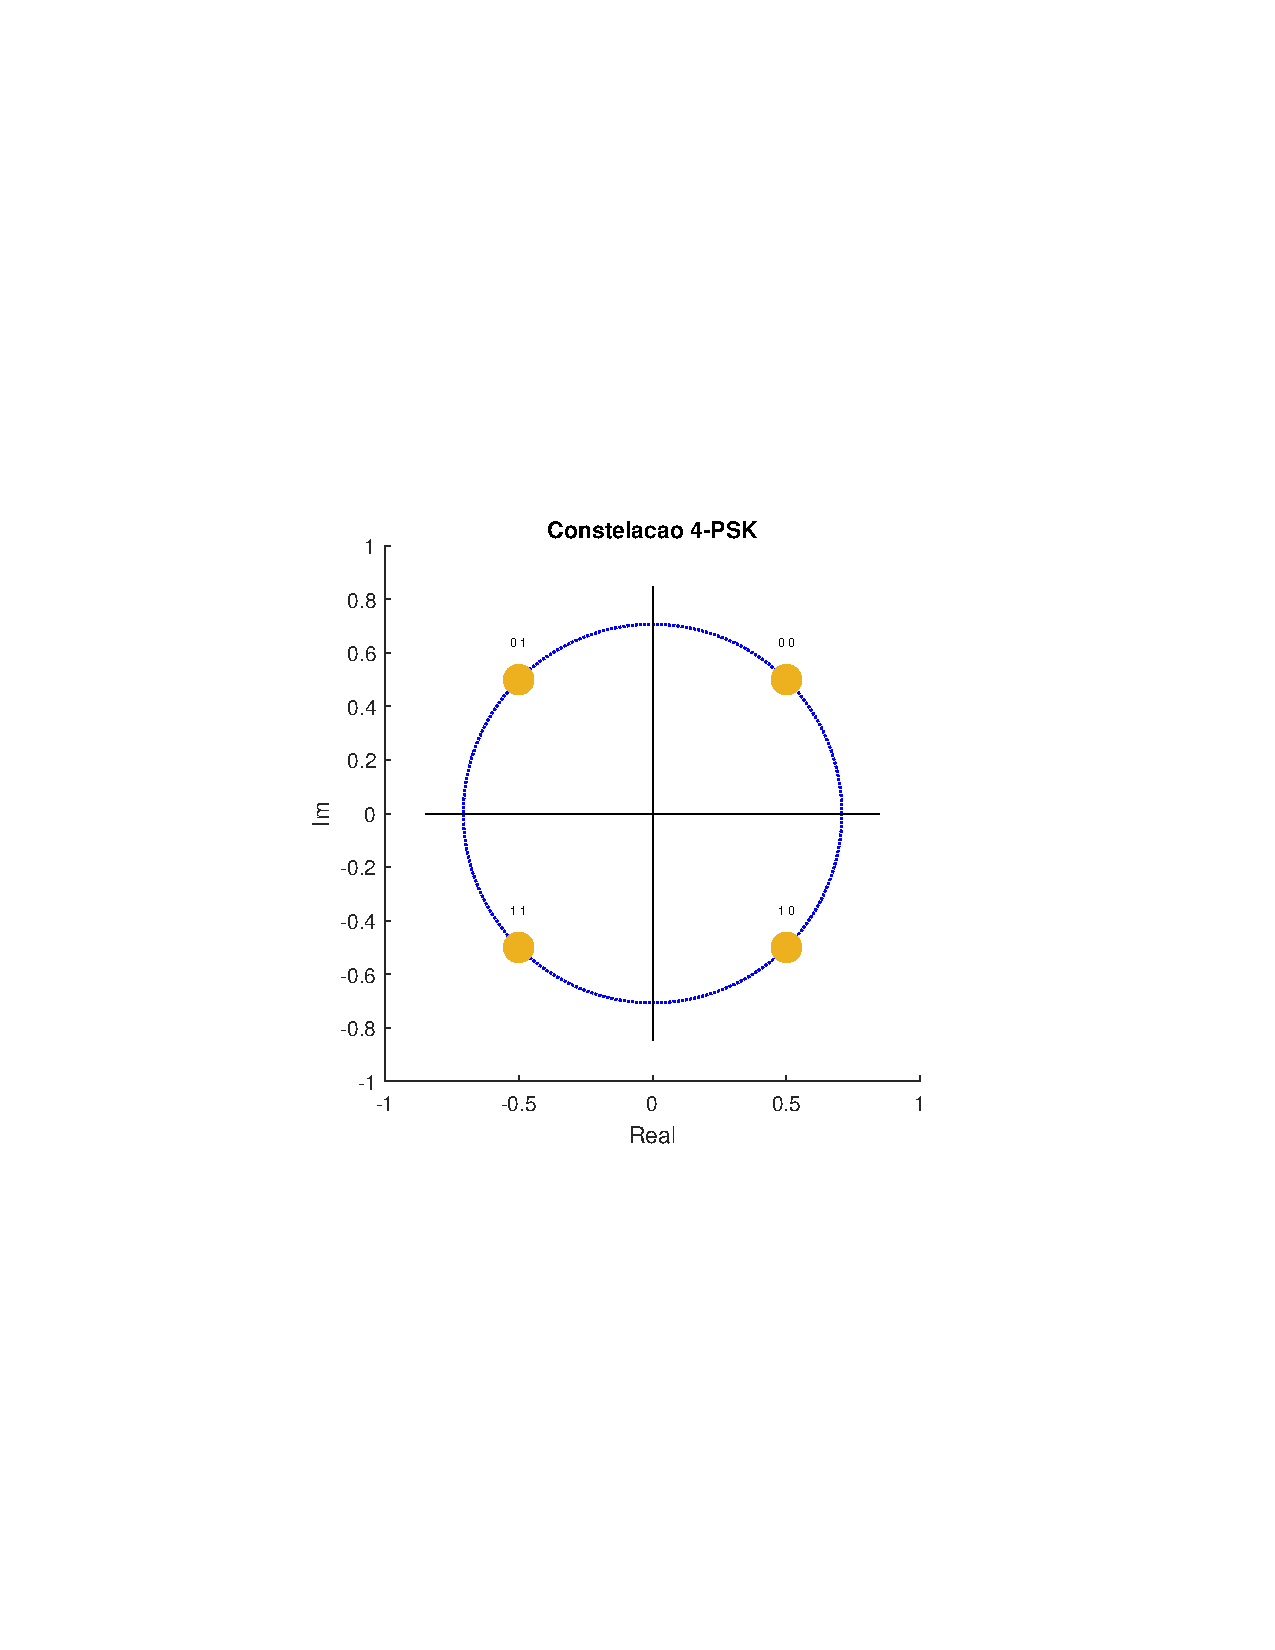
\includegraphics[width=1.0\textwidth,clip=true,trim={1.5cm 8.5cm 1.8cm 8.3cm}]{C:/Users/lukin/Documents/GitHub/Courses-HWs/Sistemas de Comunicacoes Digitais/matlab/problema4/parte1/fig/4_PSK_plot.pdf}
    \caption{Constelação $4$-PSK com codificação de Gray.}
    \label{fig:4_PSK_plot}
\end{figure}

\begin{figure}[!ht]
    \centering
    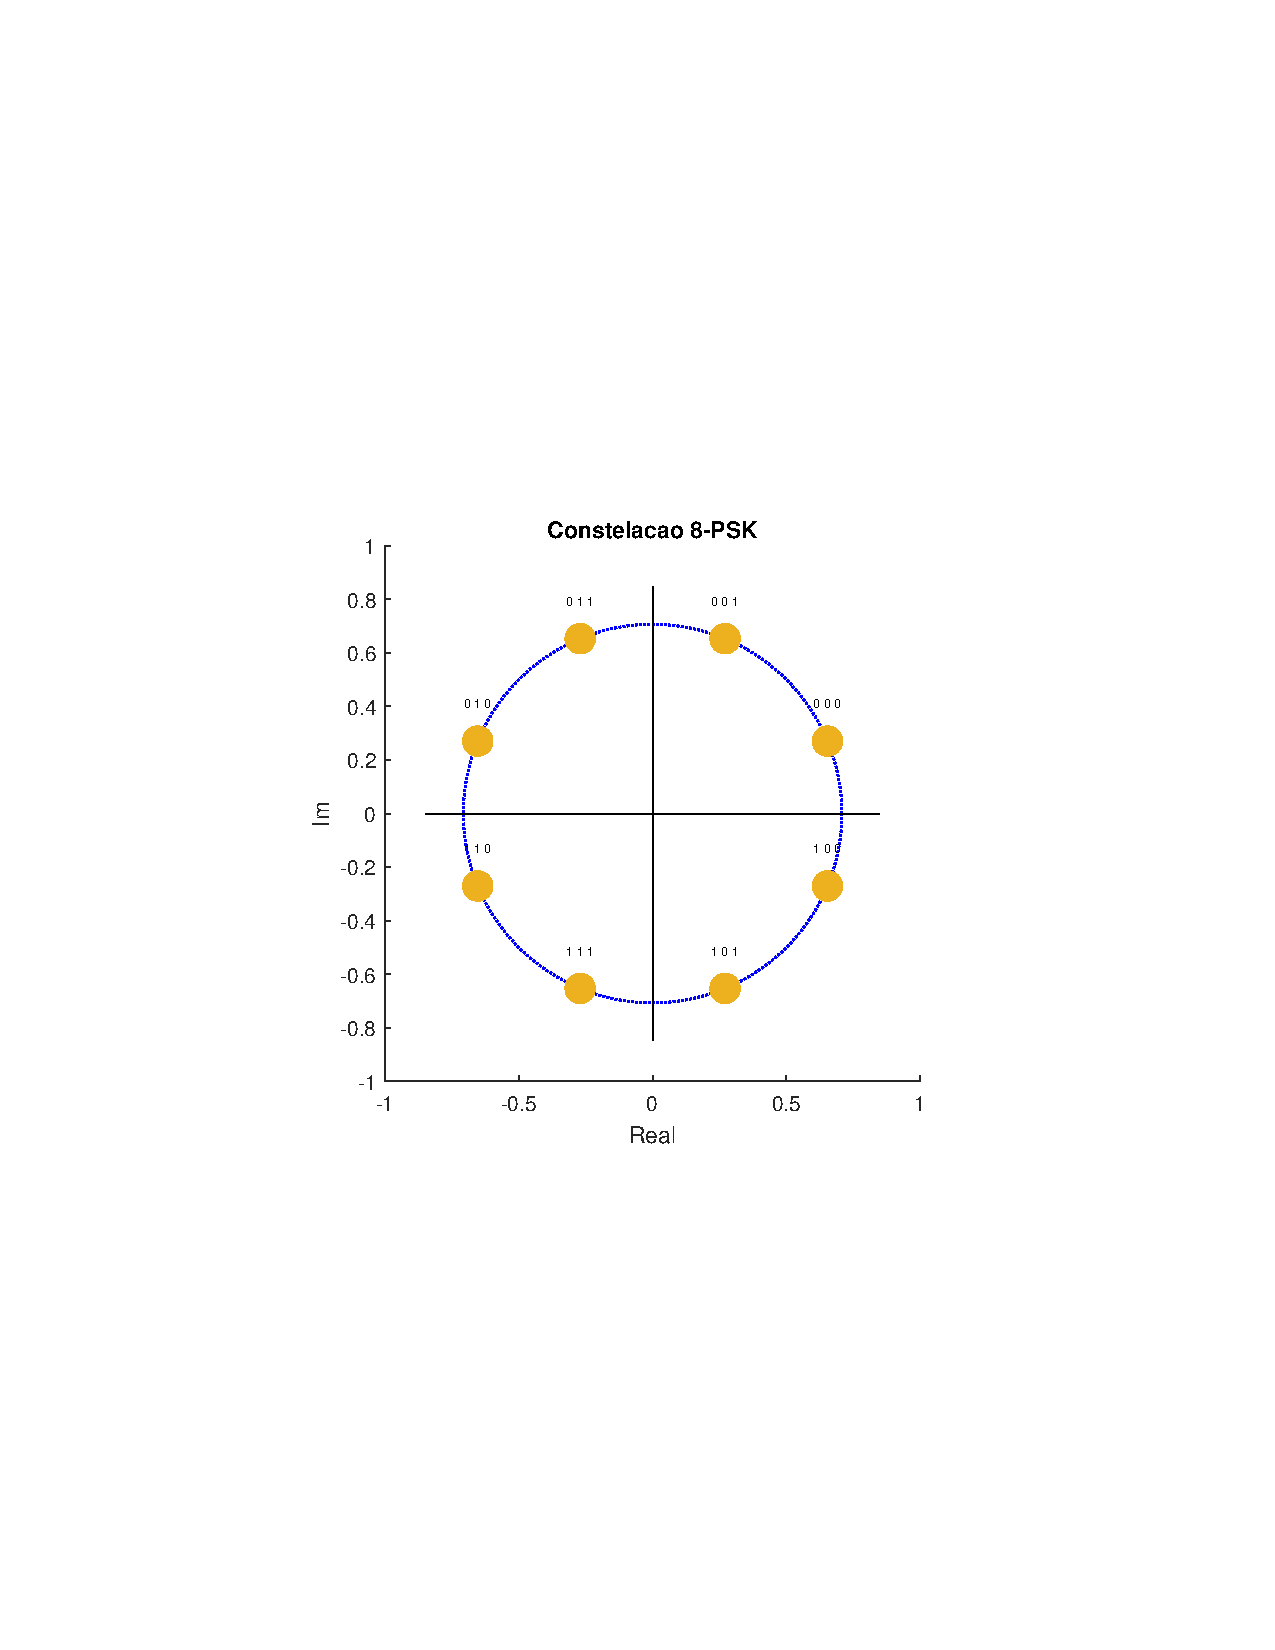
\includegraphics[width=1.0\textwidth,clip=true,trim={1.5cm 8.5cm 1.8cm 8.3cm}]{C:/Users/lukin/Documents/GitHub/Courses-HWs/Sistemas de Comunicacoes Digitais/matlab/problema4/parte1/fig/8_PSK_plot.pdf}
    \caption{Constelação $8$-PSK com codificação de Gray.}
    \label{fig:8_PSK_plot}
\end{figure}

%----------------------------------------------------------
\subsubsection{Demodulador}

A função que decodifica um símbolo tem como entrada o próprio símbolo: $A_n^{(\text{real})}$ e $A_n^{(\text{imag})}$, $M$ e $\mathcal{E}_{media}$. 

O alfabeto da constelação $M$-PSK é gerado e uma vez que estes símbolos são definidos, a área de decisão é desenhada em função de $M$ e $\mathcal{E}_{media}$. Basicamente, o símbolo selecionado é aquele que minimiza a distância euclidiana entre o símbolo recebido e o do alfabeto, como mostra a equação~\ref{eq:dist_eucliadiana} discutida nas seções anteriores.

A função que executa estes comando é a \href{https://raw.githubusercontent.com/lucasabdalah/Courses-HWs/SCD/Sistemas%20de%20Comunicacoes%20Digitais/matlab/problema1/demapping_MQAM.m}{\colorbox{cyan!10}{demapping\_MQAM.m}} e ela retorna o símbolo decodificado e os bits equivalente do alfabeto de Gray. 

% \clearpage 
%----------------------------------------------------------
\subsection{Probabilidade de Erro: \texorpdfstring{$M$}{M}-PSK}

Para calcular a probabilidade de erro $P(e)$ de cada constelação~\ref{eq:Pe_M_PSK} é necessário computar a energia da cosnstelação e do ruído, respectivamente, $E_s$ e $N_o$, que é desenvolvida em~\cite{Cecilio}.
\begin{equation}
    P(e) \approx 2Q\left( \sqrt{\frac{2 \mathcal{E}_{media}}{N_0}} \sin\left(\frac{\pi}{M}\right)\right)
    \label{eq:Pe_M_PSK}
\end{equation}

A função~\href{https://raw.githubusercontent.com/lucasabdalah/Courses-HWs/SCD/Sistemas%20de%20Comunicacoes%20Digitais/matlab/problema4/parte2/Pe_MPSK.m}{\colorbox{cyan!10}{Pe\_MPSK.m}} é utlizada para calcular a probabilidade de erro. O gráfico mostrado na figura~\ref{fig:Erro_Teorico_MPSK} mostra a probabilidade $P(e)$ caculada a partir da equação ~\ref{eq:Pe_M_PSK}, variando a \textit{SNR} de 0:2:20 dB.

\begin{figure}[!ht]
    \centering
    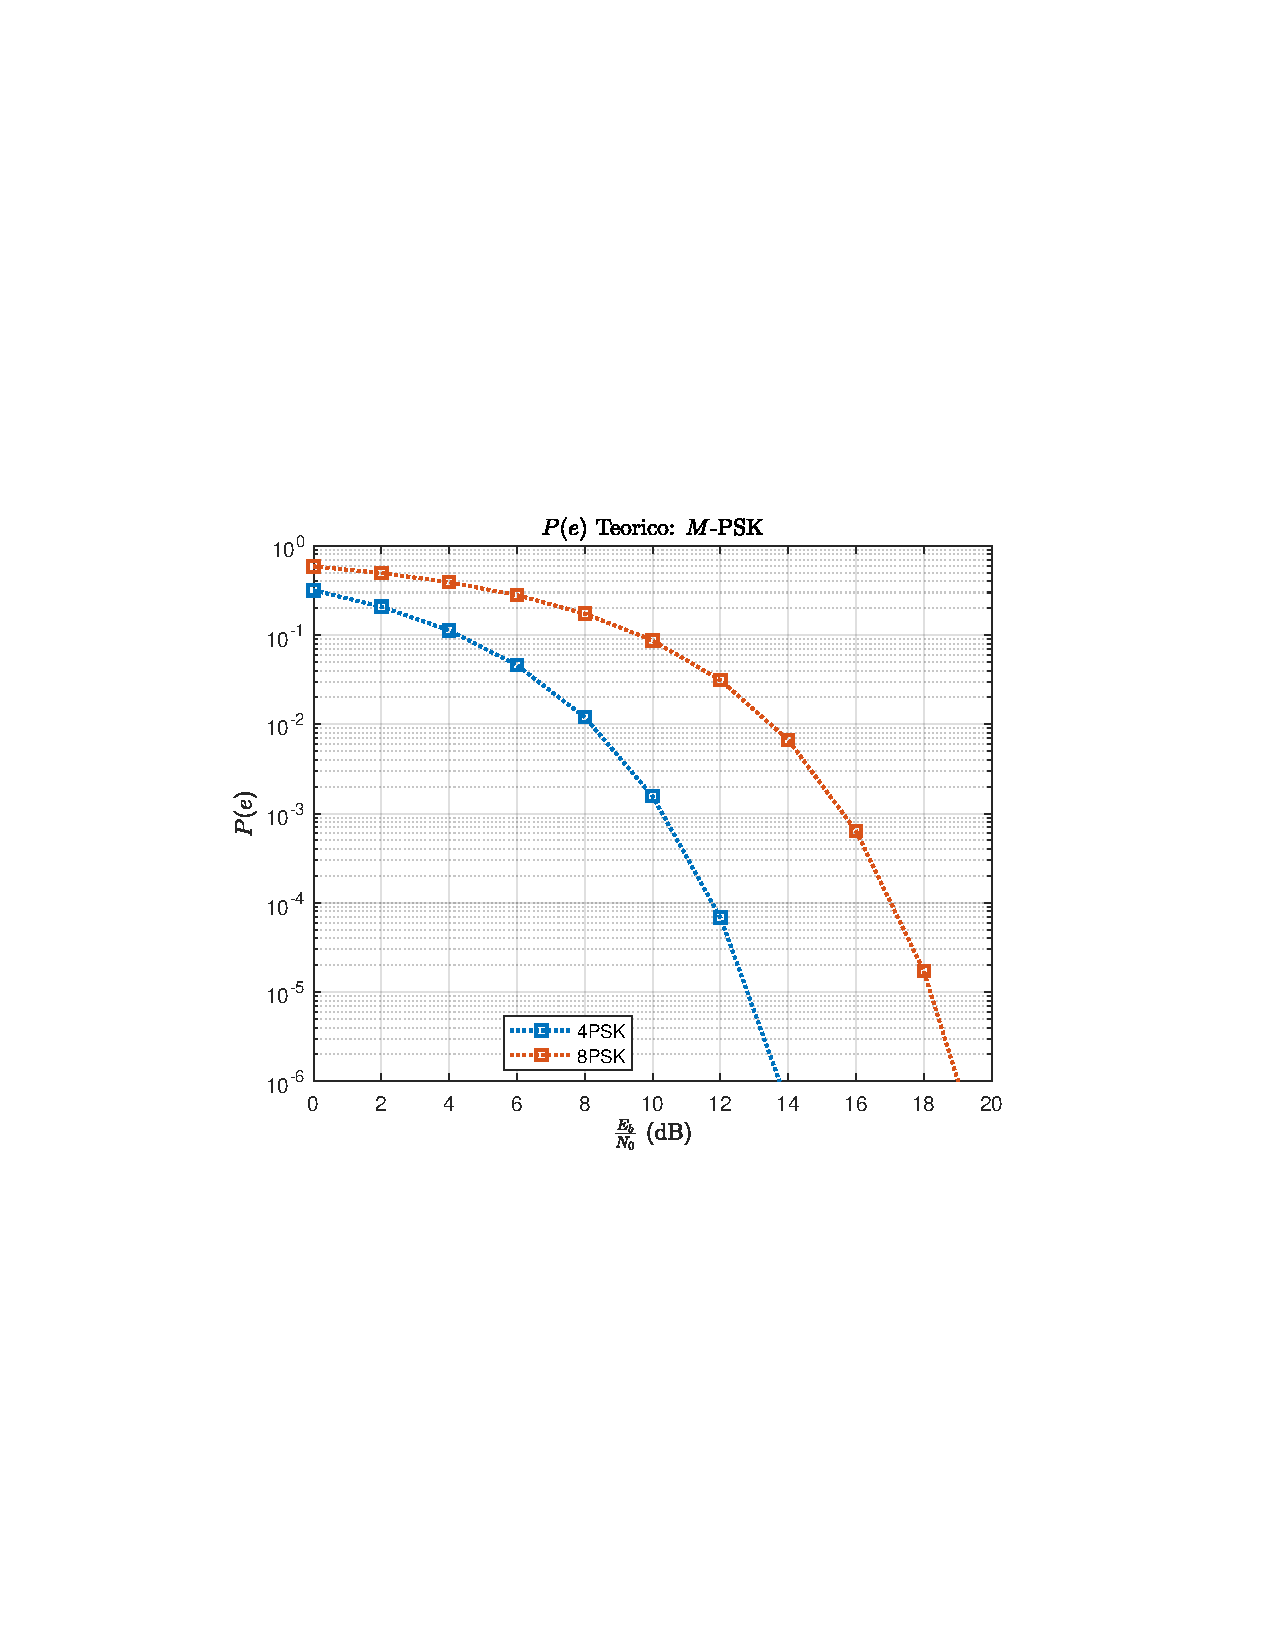
\includegraphics[width=1.0\textwidth,clip=true,trim={1.5cm 8.5cm 1.8cm 8.3cm}]{C:/Users/lukin/Documents/GitHub/Courses-HWs/Sistemas de Comunicacoes Digitais/matlab/problema4/parte2/fig/Erro_Teorico_MPSK.pdf}
    \caption{Probabilidade de erro $(P(e))$ teórico $M$-PSK.}
    \label{fig:Erro_Teorico_MPSK}
\end{figure}

\clearpage

\subsection{Canal RAGB: \texorpdfstring{$M$}{M}-PSK}
\subsubsection{Modelo}


Seguindo o mesmo modelo utilizado para o caso $M$-QAM da equação~\ref{eq:AWGM_Model}, o modelo $M$-PSK, com $M = 4$ recebe uma sequência de símbolos com SNR de 25dB gerados no script \href{https://raw.githubusercontent.com/lucasabdalah/Courses-HWs/SCD/Sistemas%20de%20Comunicacoes%20Digitais/matlab/problema4/parte3/script_AWGN.m}{\colorbox{gray!10}{\color{red} script\_AWGN.m}} para ilustrar a implementação a passagem dos símbolos pelo canal, como mostrado na figura~\ref{fig:4PSK_25dB}.

\begin{figure}[!ht]
    \centering
    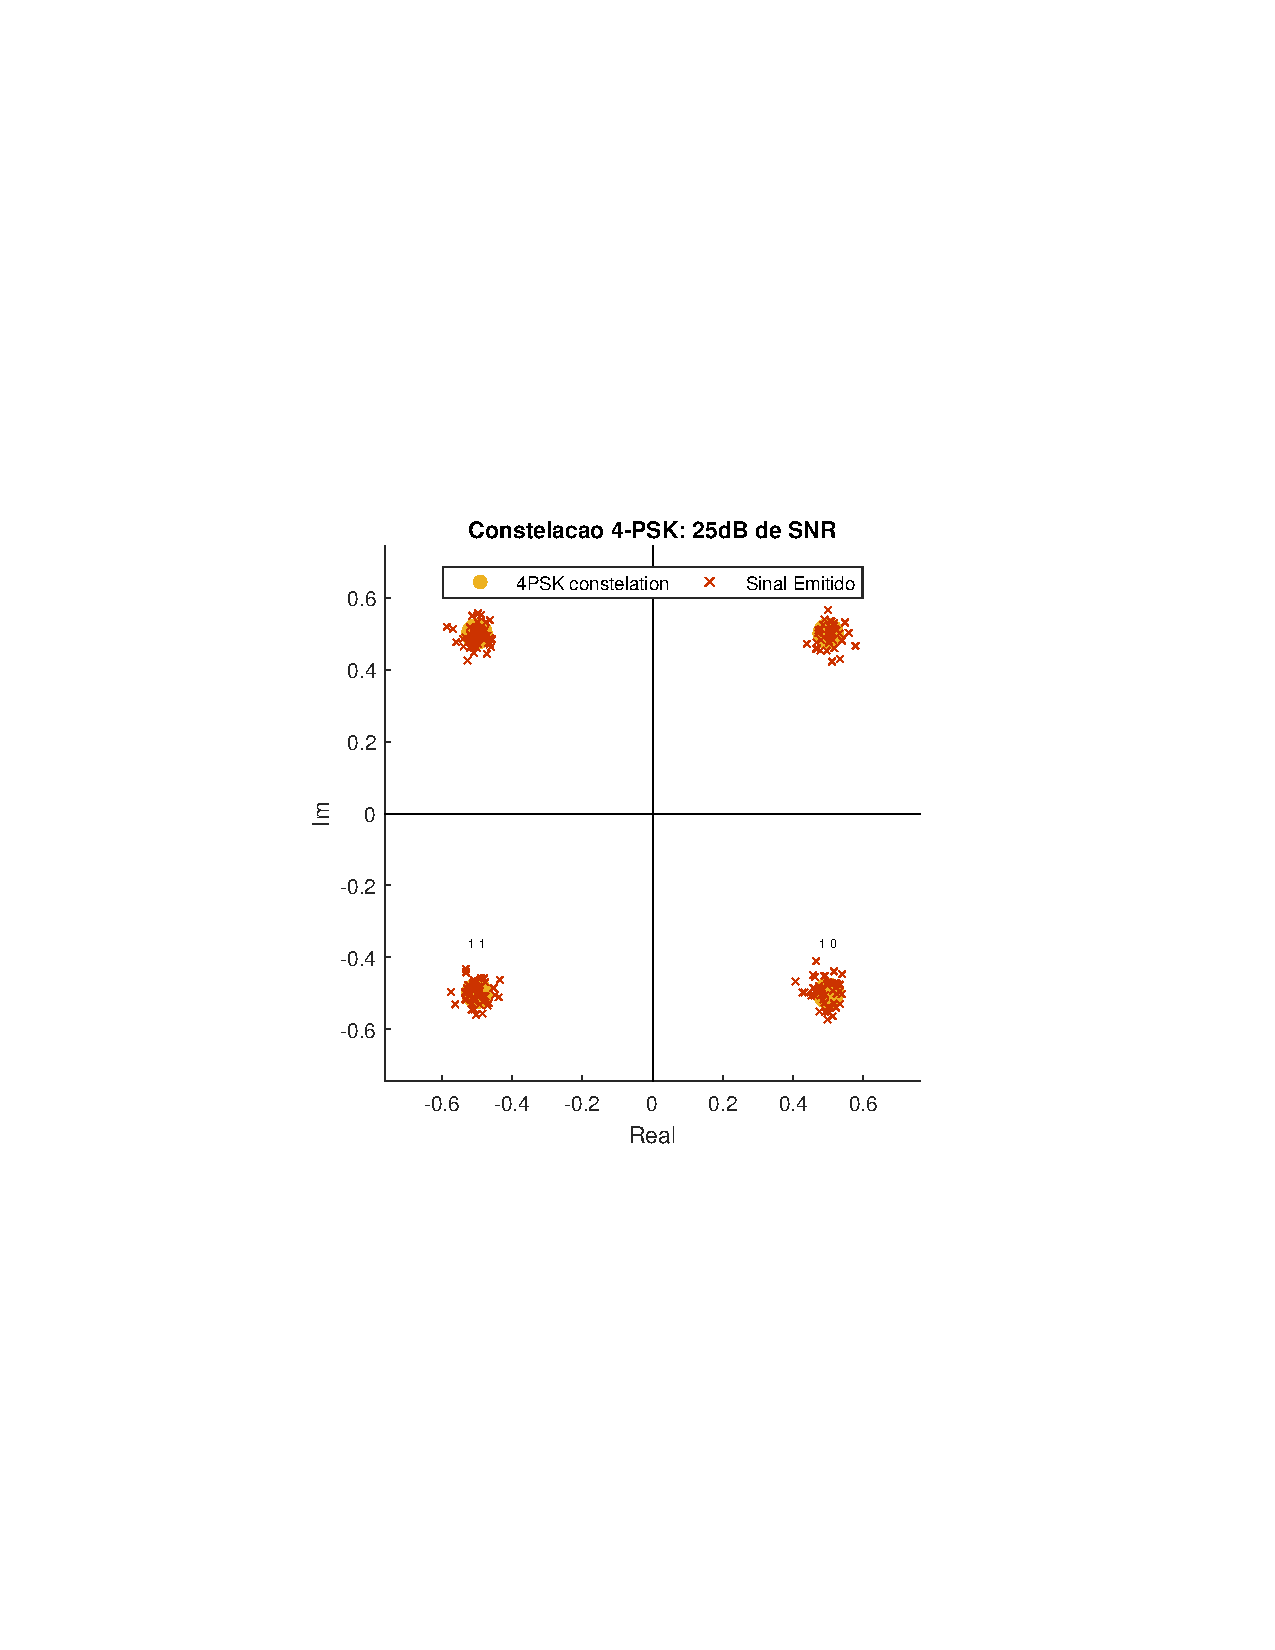
\includegraphics[width=1.0\textwidth,clip=true,trim={1.5cm 8.5cm 1.8cm 8.3cm}]{C:/Users/lukin/Documents/GitHub/Courses-HWs/Sistemas de Comunicacoes Digitais/matlab/problema4/parte3/fig/4PSK_25dB.pdf}
    \caption{Simulação de transmissão $4$-PSK, com \textit{SNR} de 25dB..}
    \label{fig:4PSK_25dB}
\end{figure}

\begin{figure}[!ht]
    \centering
    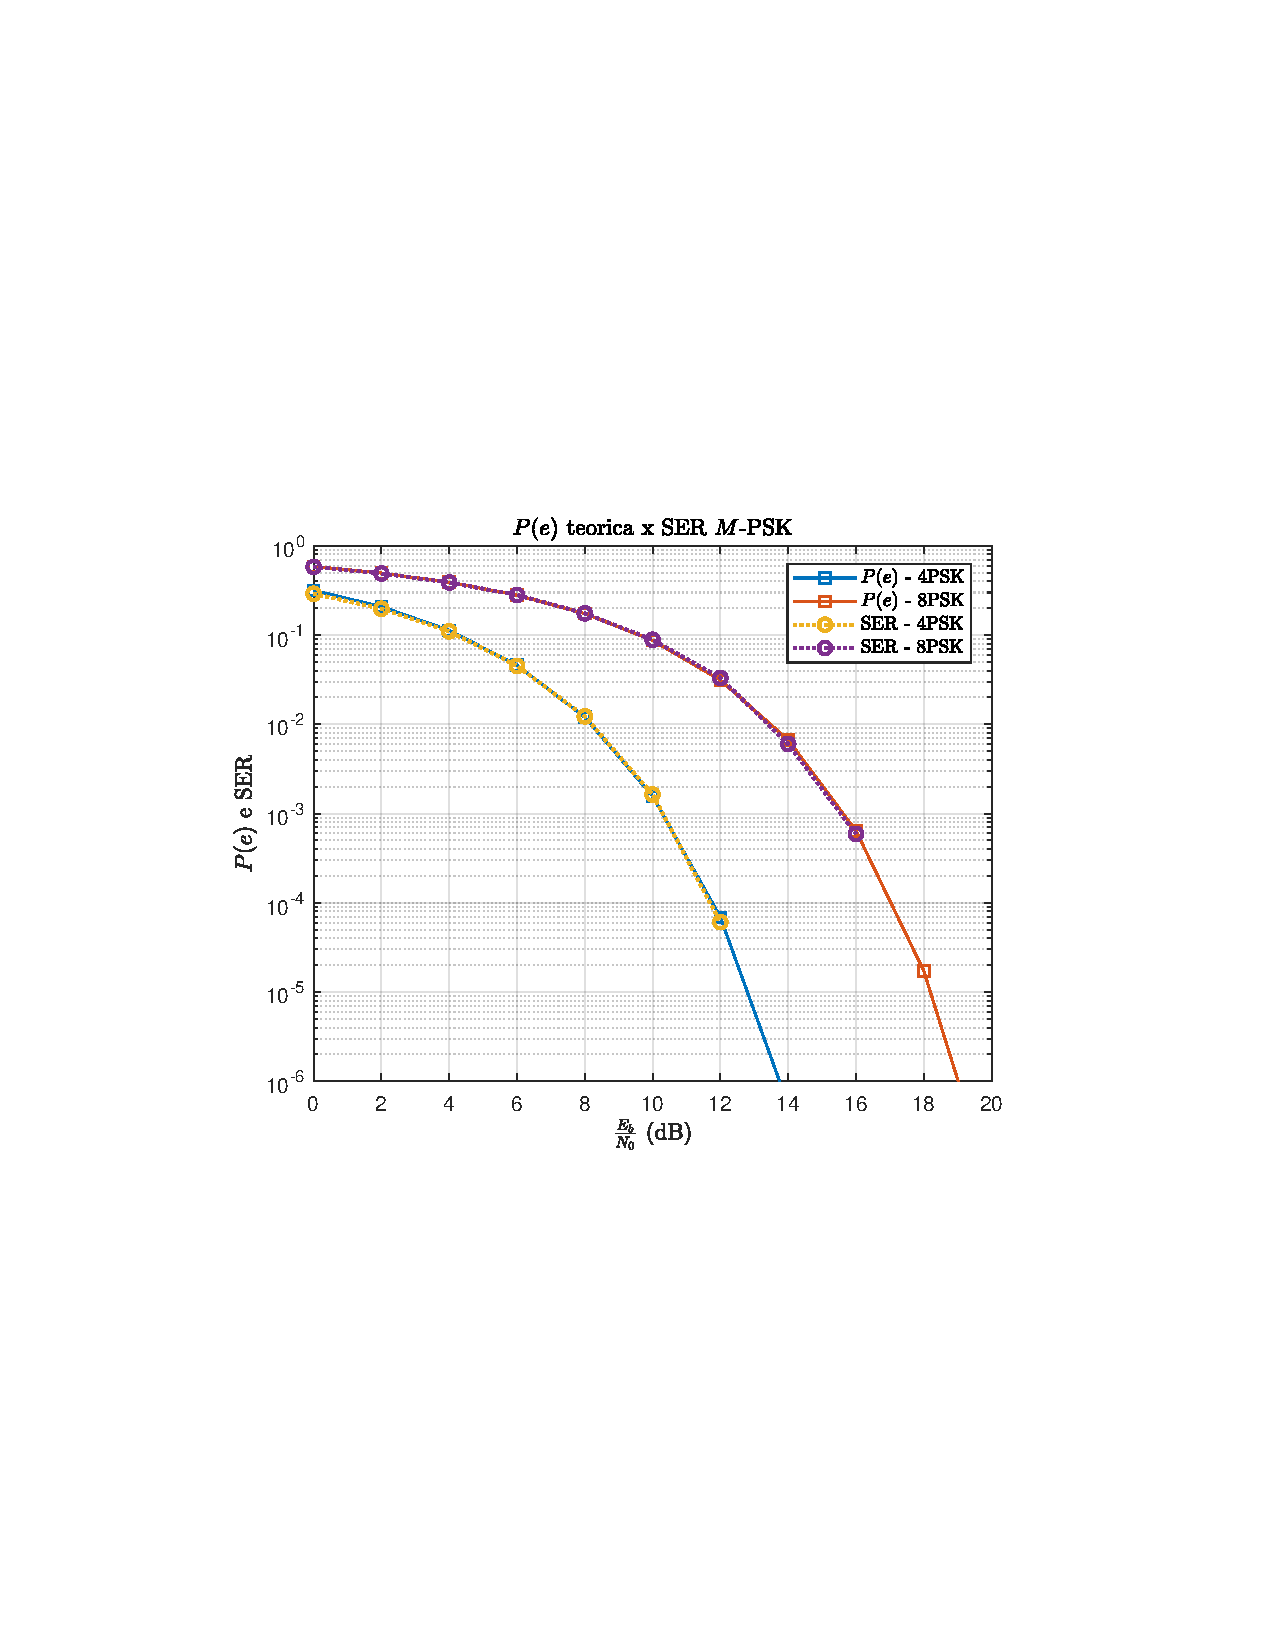
\includegraphics[width=1.0\textwidth,clip=true,trim={1.5cm 8.5cm 1.8cm 8.3cm}]{C:/Users/lukin/Documents/GitHub/Courses-HWs/Sistemas de Comunicacoes Digitais/matlab/problema4/parte3/fig/Erro_teoricaxAWGN_MPSK.pdf}
    \caption{Probabilidade teórica de erro vs. simulação de transmissão $M$-PSK em canal RAGB.}
    \label{fig:Erro_teoricaxAWGN_MPSK}
\end{figure}
